\newpage
\section{Modeling NASA-TLX Weighted Scores and Subscales}
\label{apdx:model_tlx}
In this section, we first describe the modeling approach for the NASA-TLX weighted scores and subscales, and then present all subscale results.

\subsection{Modeling Approach}
We modeled the NASA-TLX weighted scores and subscales using a hierarchical Bayesian ordinal regression model. 

\subsubsection{Dependent variables}
\paragraph{NASA-TLX weighted scores} are transformed from a continuous $0$–$100$ scale to cognitive levels: low, medium, somewhat high, high, and very high, as described by~\textcite{hart1988development}. This transformation helps the model adapt to sparse data. In our study, there were no participants who expressed "low" or "very high"; thus, we modeled the predictive variables as "medium," "somewhat high," and "high."

\paragraph{NASA-TLX subscale ratings} are transformed into ordinal groups using using minimum frequency binning~\cite{frank2001simple}. Minimum frequency binning involves grouping adjacent response categories until each bin meets a predefined minimum number of observations. The subscale uses a 21-point Likert scale, with 40 participants, it makes the ordinal data very sparse. Minimum frequency binning mitigates this allowing similiar number of participants in each bin. We applied weighted bins across all participants within the same subscale, ensuring that each bin contained at least 10 participants.

\subsubsection{Independent Variables}
For this model, we used three independent variables: length ($\gamma_i$), interface type ($\beta_I$), and the interaction between the two ($\phi_{ij}$). Length, categorized as "low" and "short," was modeled as an ordinal variable, as shown in Equation~\ref{eq:cog_ordinal}. Since there are only two categories, this approach allowed us to model the baseline length effect and the added effect of the longer length. Interface types were set up with hyperpriors, from which the interfaces were drawn. The interaction effect used a non-centered parameterization constrained by an LKJ prior to account for correlations, as described in Equation~\ref{eq:cog_lkj}. Weakly informed priors were used for all parameters, as shown in Equations~\ref{eq:cog_prior_1},~\ref{eq:cog_prior_2}, and~\ref{eq:cog_prior_3}.

\subsubsection{Overall Model}
We modeled the dependent variables using an Ordered Logistic (Equation~\ref{eq:cog_main}). The Ordered Logistic model is particularly suited for ordinal outcome variables, where the categories have a natural order but the intervals between them are not necessarily equal. This model has two input parameters: $\eta_i$ and $\tau$. $\eta_i$ is the latent predictor derived from a regression equation that incorporates the independent variables, demonstrated as Equation~\ref{eq:cog_regression}. The purpose of it, intuitively, is to model how specific independent variables pushes this latent value towards a higher or lower category. $\tau$ as modeded by Equation~\ref{eq:cog_orderedTransfrom} are the cutpoints that demarcate the boundaries between the ordinal categories. This cutpoint draws from a normal distribution and being transformed to ensure that the thresholds are ordered. The Ordered Logistic model then compares $\eta_i$ to $\tau$ to determine the probability of the observed outcome $y_i$ falling into a specific ordinal category.


\begin{align}
    y_i &\sim \text{OrderedLogistic}(\eta_i, \boldsymbol{\tau}) \label{eq:cog_main}\\
    \eta_i &= \alpha + \gamma_i + \beta_I[I_i] + \phi_{ij} \label{eq:cog_regression}\\
    \boldsymbol{\tau} &\sim \text{OrderedTransform}(\mathcal{N}(0, 1)^{K-1}) \label{eq:cog_orderedTransfrom} \\
    \gamma_i &= \mu_L + \beta_L \cdot L_i \label{eq:cog_ordinal} \\
    \phi_{ij} &= L_{\Omega} \cdot (\sigma_{\phi} \odot z_{\phi}) \label{eq:cog_lkj}
\end{align}


\paragraph{Priors}
We specify priors for all model parameters. The priors are defined as follows:
\begin{align}
    \mu_{L}, \mu_{\beta_L}, \mu_{\beta_I} &\sim \mathcal{N}(0, 1), \quad \sigma_{\beta_L}, \sigma_{\beta_I} \sim \text{Exponential}(1) \label{eq:cog_prior_1} \\
    \beta_L &\sim \mathcal{N}(\mu_{\beta_L}, \sigma_{\beta_L}), \quad \beta_I \sim \mathcal{N}(\mu_{\beta_I}, \sigma_{\beta_I}) \label{eq:cog_prior_2} \\
    L_{\Omega} &\sim \text{LKJ}(2), \quad \sigma_{\phi} \sim \text{Exponential}(1), \quad z_{\phi} \sim \mathcal{N}(0, 1) \label{eq:cog_prior_3} 
\end{align}

In Equation~\ref{eq:cog_prior_1} and \ref{eq:cog_prior_2} we present the hyperpriors reflecting our belief that the mean effects of length and interface are centered around zero with a standard deviation of one. Hyperpriors were used to enable partial pooling where information is shared across different levels of the interface type, improving estimation accuracy especially in cases with limited data per group. Equation~\ref{eq:cog_prior_3} describes the correlation metrix used for the interaction effect. The LKJ prior of 2 refers to a moderate correlation without being too restrictive allowing the model to learn appropriate levels of interaction terms. $\sigma_{\phi}$ ensuring that the variability of the interaction effects remains positive and allowing the model to flexibly adapt to different levels of interaction strength and $z_{\phi}$ were assigned to serves as a standardized component that, when scaled by $\sigma_{\phi}$ with the correlation matrix $L_{\Omega}$ captures the magnitude and the dependencies of the interaction terms effectively.


\subsubsection{Model Results}
We conducted the Bayesian analysis using NumPyro, a widely used framework for Bayesian inference. We used Markov Chain Monte Carlo (MCMC) sampling, a method commonly applied in Bayesian inference. All the models showed that the Gelman-Rubin statistic ($\hat{R}$) parameters were equal to 1 across two chains, indicating that the multiple sampling chains converged. We present each subscale result and provide a short description of these results.

% Section for Mental subscale
\subsubsection{Mental Subscale}
Figure~\ref{fig:bayesian_mental_subscale} shows pairwise bayesian results from mental demand highlighted 70.4\% of posterier probaility that participants in the long two-phase condition had a higher mental demand compared to the short two-phase condition. On the other hand, the short text condition had a 74.5\% posterior probability of having a higher mental demand compared to the short two-phase condition. This is additional evidence that prompted us to believe that the participants in the short two-phase participants benifited from the organization phase. The sheer number of added options in the long two-phase condition may have added additional demand to participants, leading to higher mental demand.

\begin{figure}[h!]
    \centering
    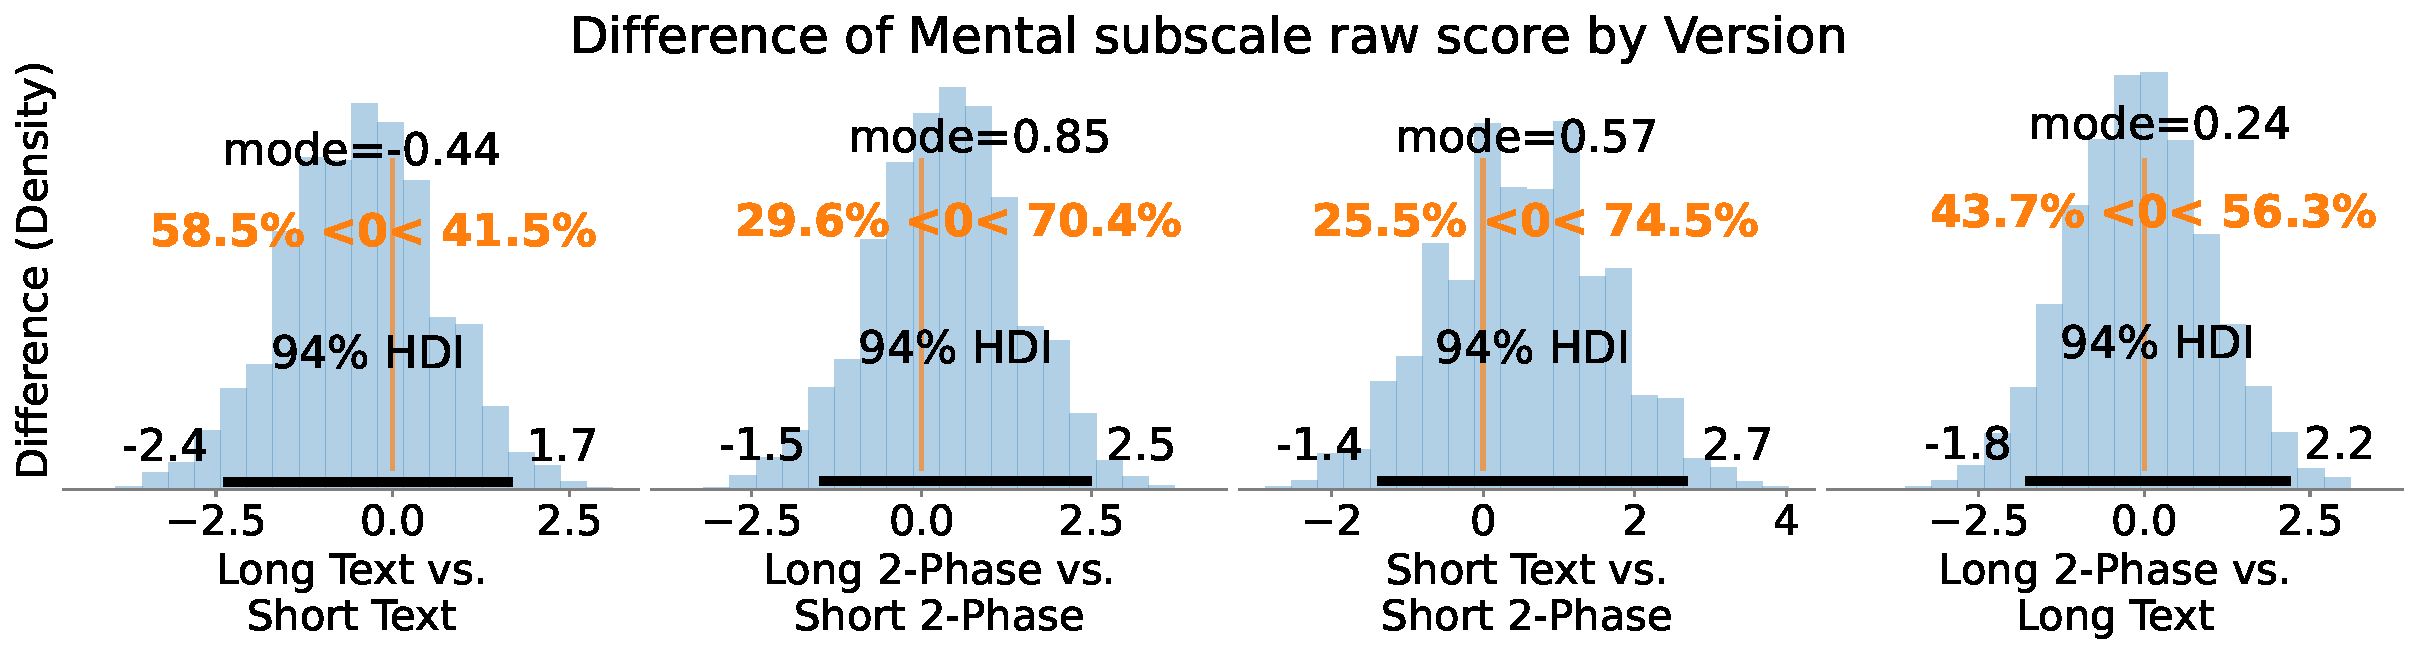
\includegraphics[width=\textwidth]{content/image/cog/Mental_cog_diff_single_row.pdf}
    \caption{Differences in the mental subscale scores by version.}
    \label{fig:bayesian_mental_subscale}
\end{figure}

% Section for Physical subscale
\subsubsection{Physical Subscale}
Figure~\ref{fig:bayesian_physical_subscale} shows the pairwise comparison of the physical subscale. Noteable results shows that there is a 86.1\% posterior probability that the long text condition had a lesser physical demand compared to the short text condition. This is counter intuitive as the long text participants actually traversed much higher edit distances. We are not clear what prompted their self reported value and requires future research. 

\begin{figure}[h!]
    \centering
    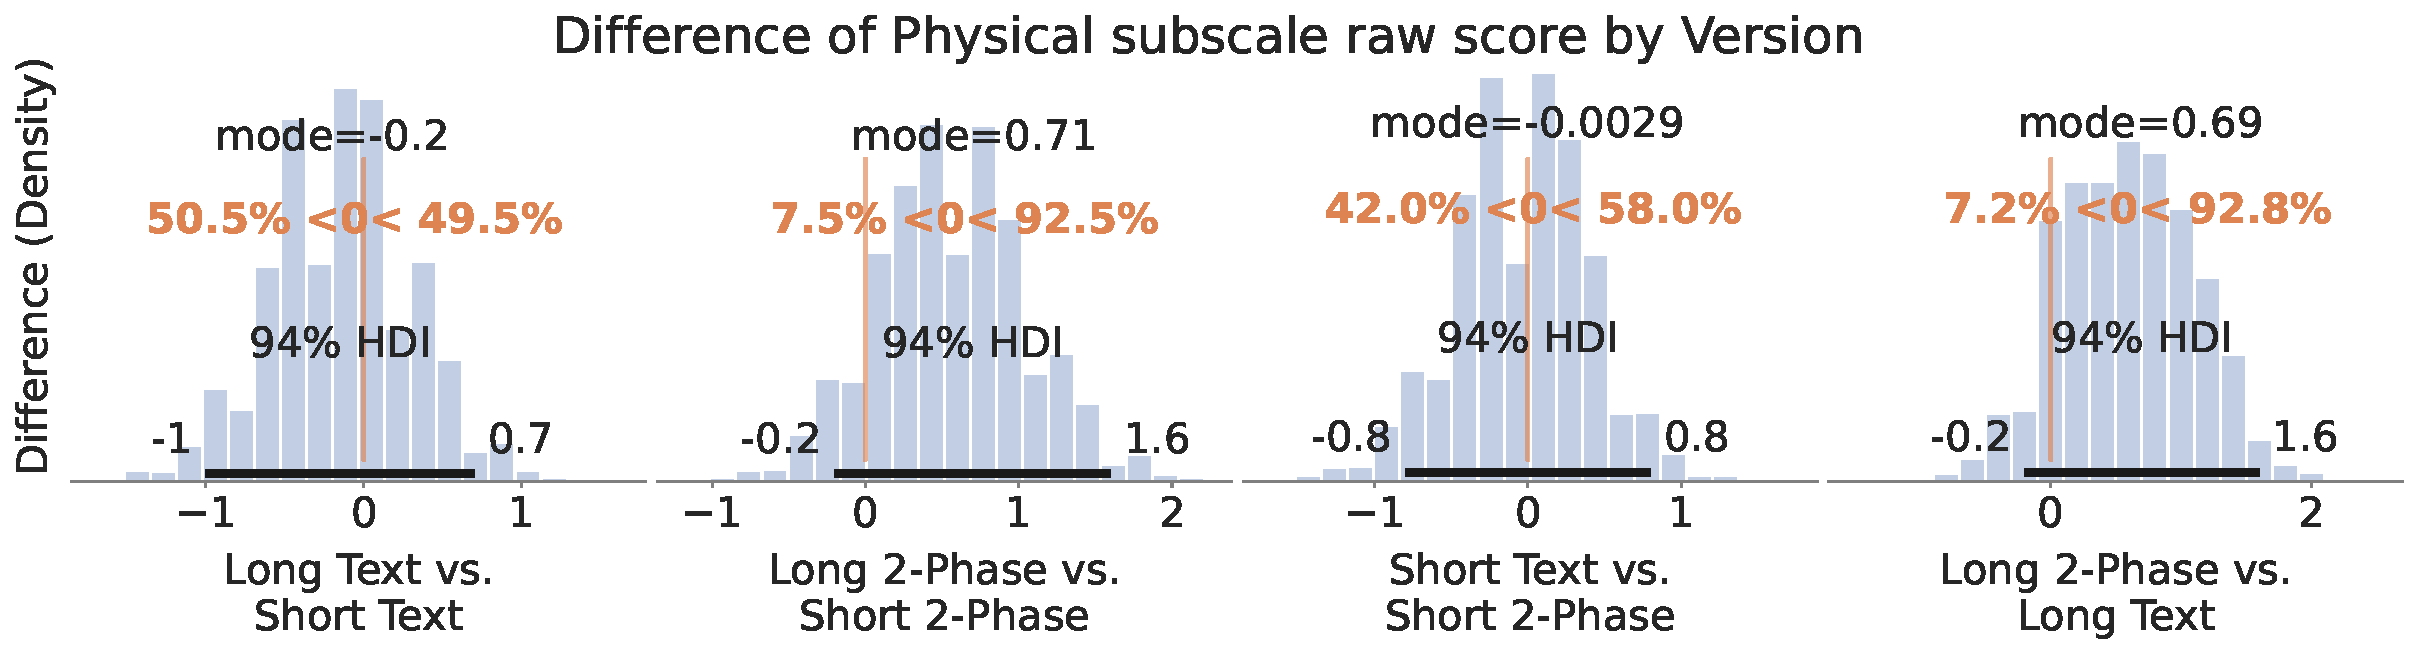
\includegraphics[width=\textwidth]{content/image/cog/Physical_cog_diff_single_row.pdf}
    \caption{Differences in the physical subscale scores by version.}
    \label{fig:bayesian_physical_subscale}
\end{figure}

% Section for Temporal subscale
\subsubsection{Temporal Subscale}
\label{sec:temporal_subscale_bayesian}
Figure~\ref{fig:bayesian_temporal_subscale} shows the pairwise comparison of the temporal subscale. The results show that the long two-phase condition once again had a 74.6\% posterior probability of having a lower temporal demand compared to the short text condition. Conversely, participants in the long two-phase condition had a 71.1\% posterior probability of having a higher temporal demand compared to the short two phase condition, reflecting the longer time they took to complete the survey questions. We believe that the lower temporal demand in the long two-phase condition are potential indicators of participant's satisficing behavior.

\begin{figure}[h!]
    \centering
    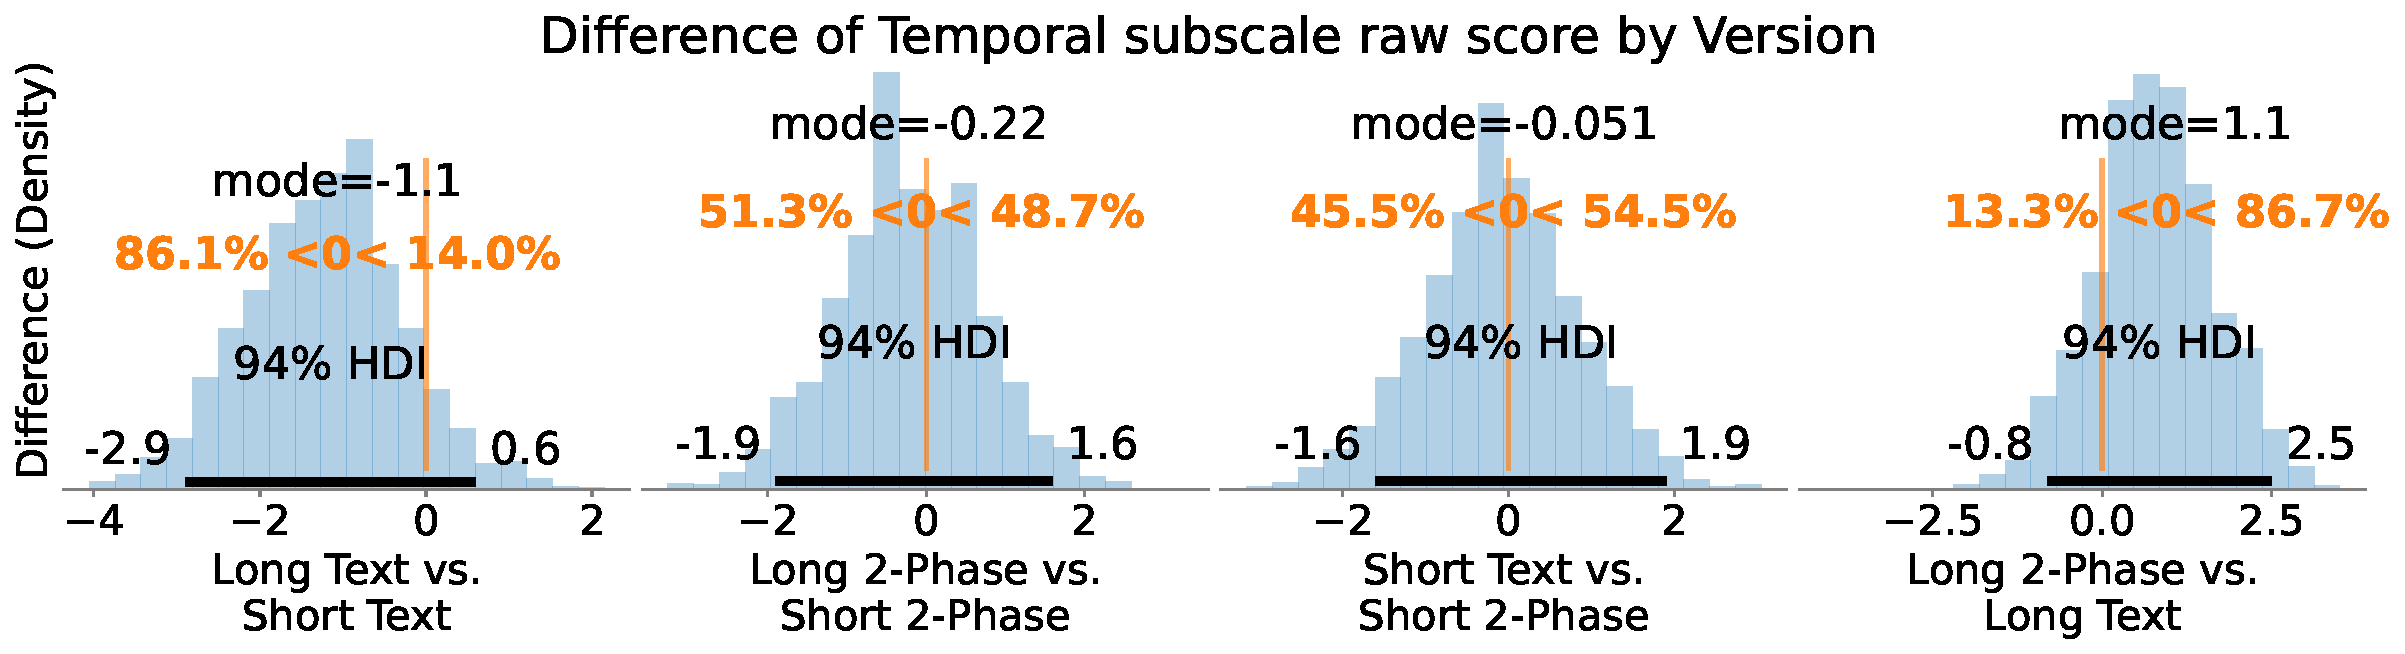
\includegraphics[width=\textwidth]{content/image/cog/Temporal_cog_diff_single_row.pdf}
    \caption{Differences in the temporal subscale scores by version.}
    \label{fig:bayesian_temporal_subscale}
\end{figure}

% Section for Performance subscale
\subsubsection{Performance Subscale}
We omit the pairwise comparison of the performance subscale due to the mixed signals. We focused on the qualitative results analyzed in the main text.
% Figure~\ref{fig:bayesian_performance_subscale} shows the pairwise comparison of the performance subscale. The results showed mixed signals. Thus, we focused on the qualitative results analyzed in the main text.

% \begin{figure}[h!]
%     \centering
%     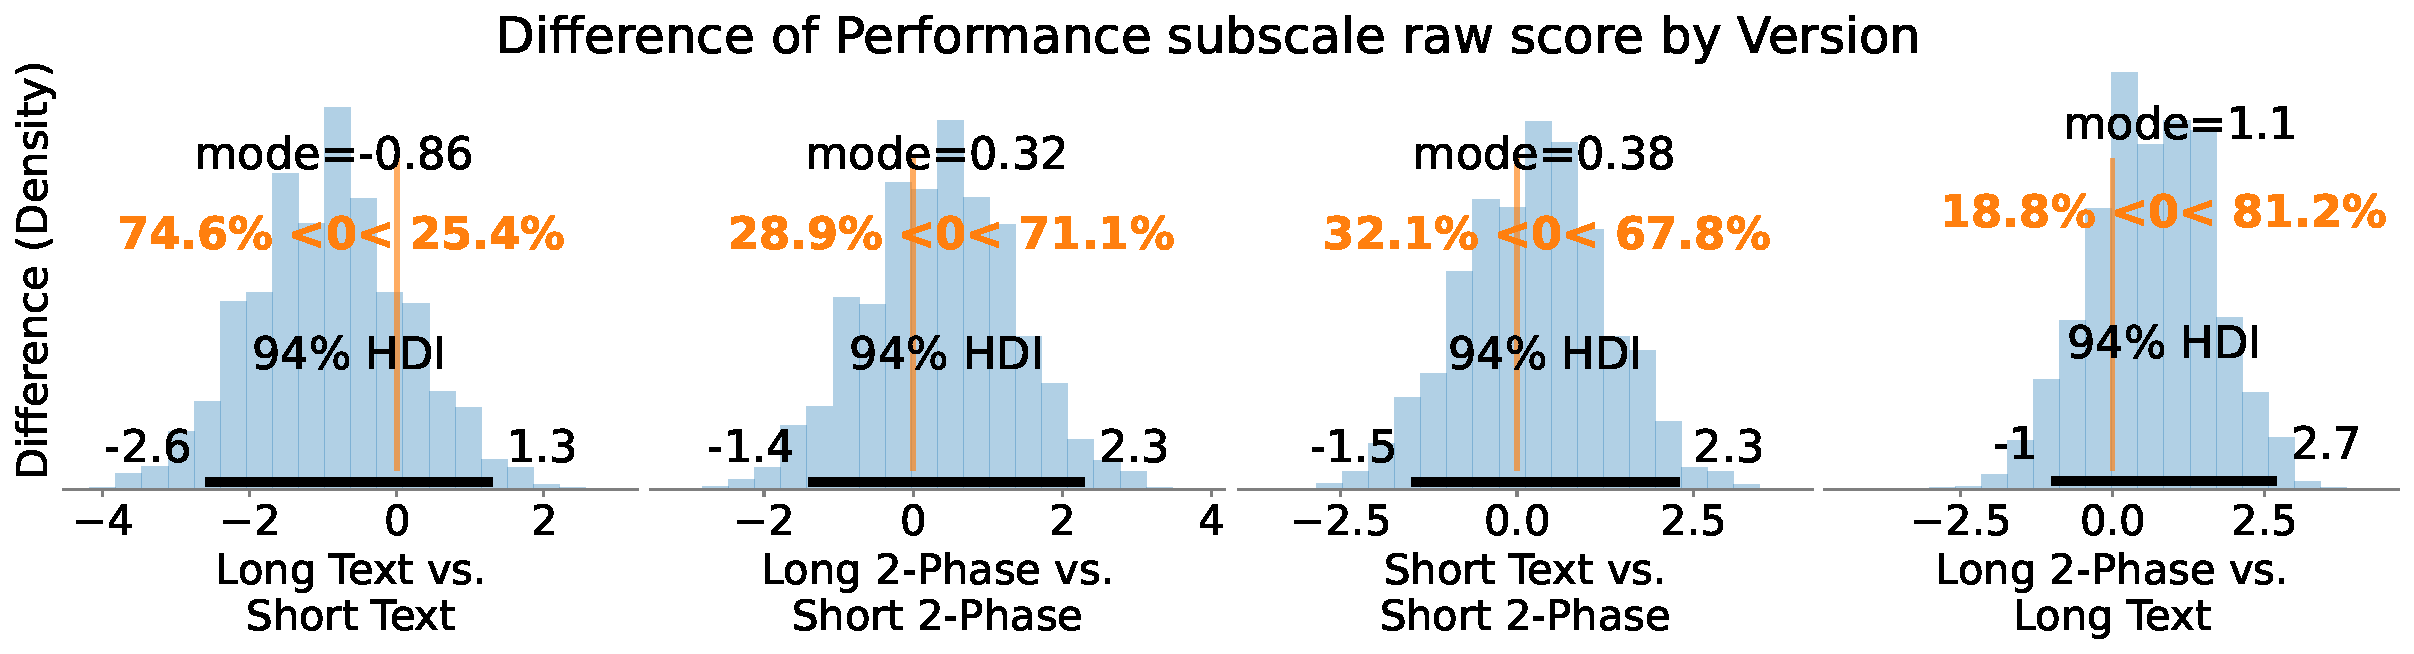
\includegraphics[width=\textwidth]{content/image/cog/Performance_cog_diff_single_row.pdf}
%     \caption{Differences in the performance subscale scores by version.}
%     \label{fig:bayesian_performance_subscale}
% \end{figure}

% Section for Effort subscale
\subsubsection{Effort Subscale}
We omit the pairwise comparison of the effort subscale due to its similarity to the mental demand subscale. 

% \begin{figure}[h!]
%     \centering
%     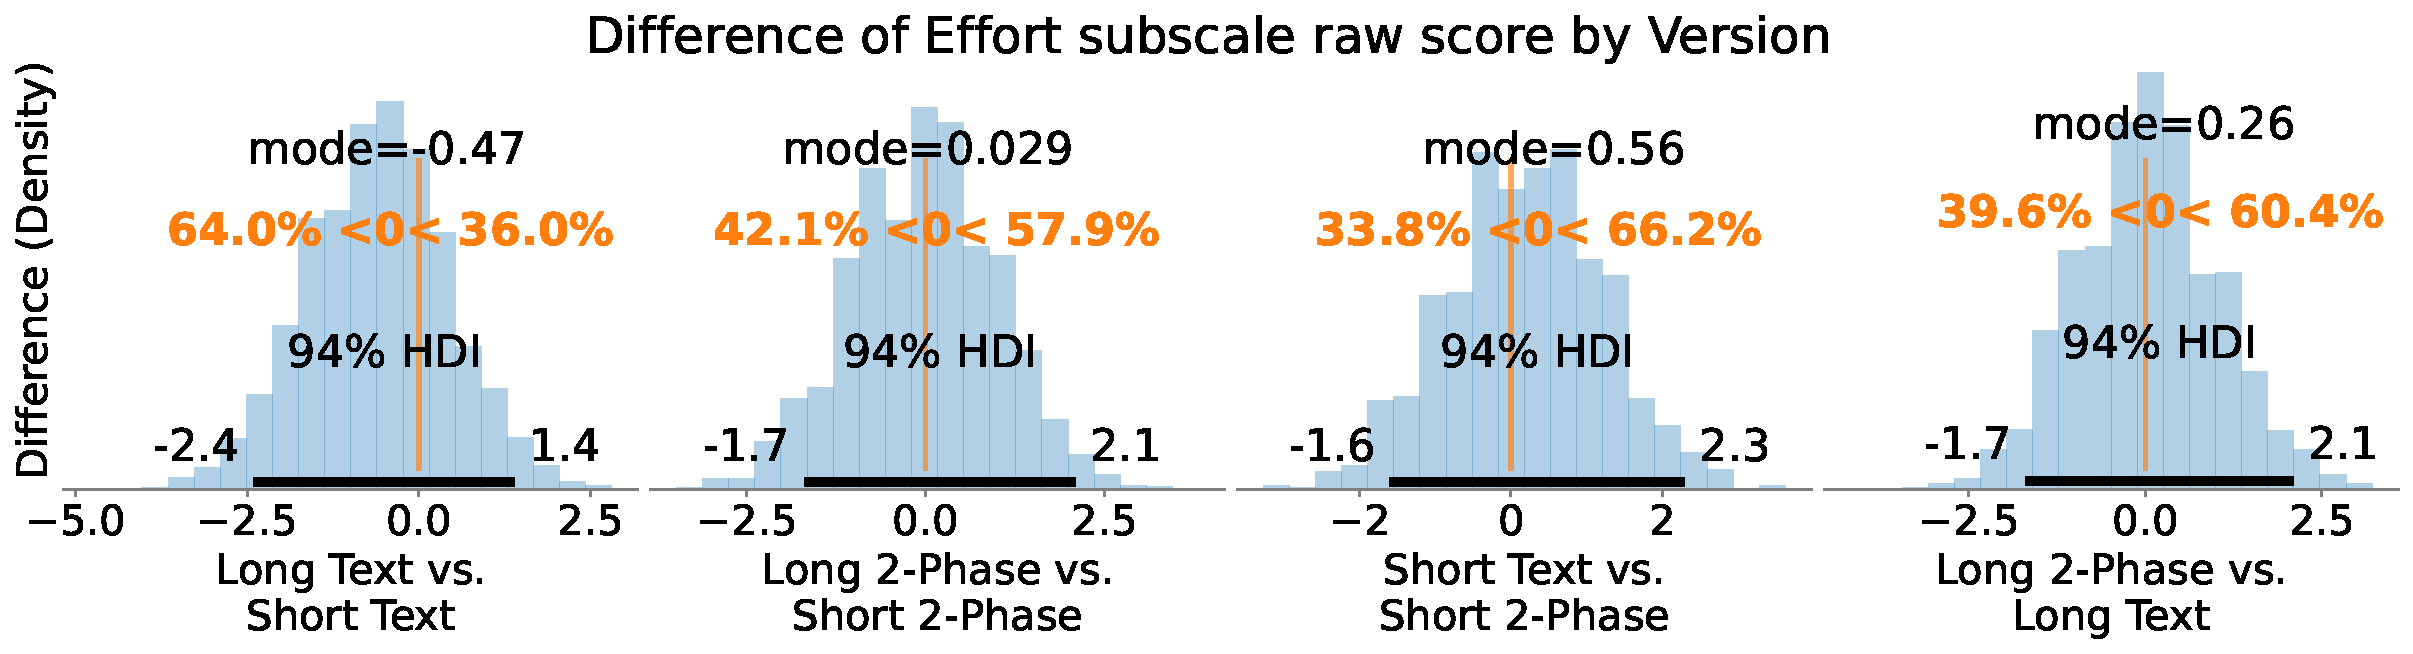
\includegraphics[width=\textwidth]{content/image/cog/Effort_cog_diff_single_row.pdf}
%     \caption{Differences in the effort subscale scores by version.}
%     \label{fig:bayesian_effort_subscale}
% \end{figure}

% Section for Frustration subscale
\subsubsection{Frustration Subscale}
Figure~\ref{fig:bayesian_frustration_subscale} shows the pairwise comparison of the frustration subscale. The results show that the long two-phase condition had a 68.3\% posterior probability of having a higher frustration compared to the short two-phase condition, likey due to the added number of options to assess. 

\begin{figure}[h!]
    \centering
    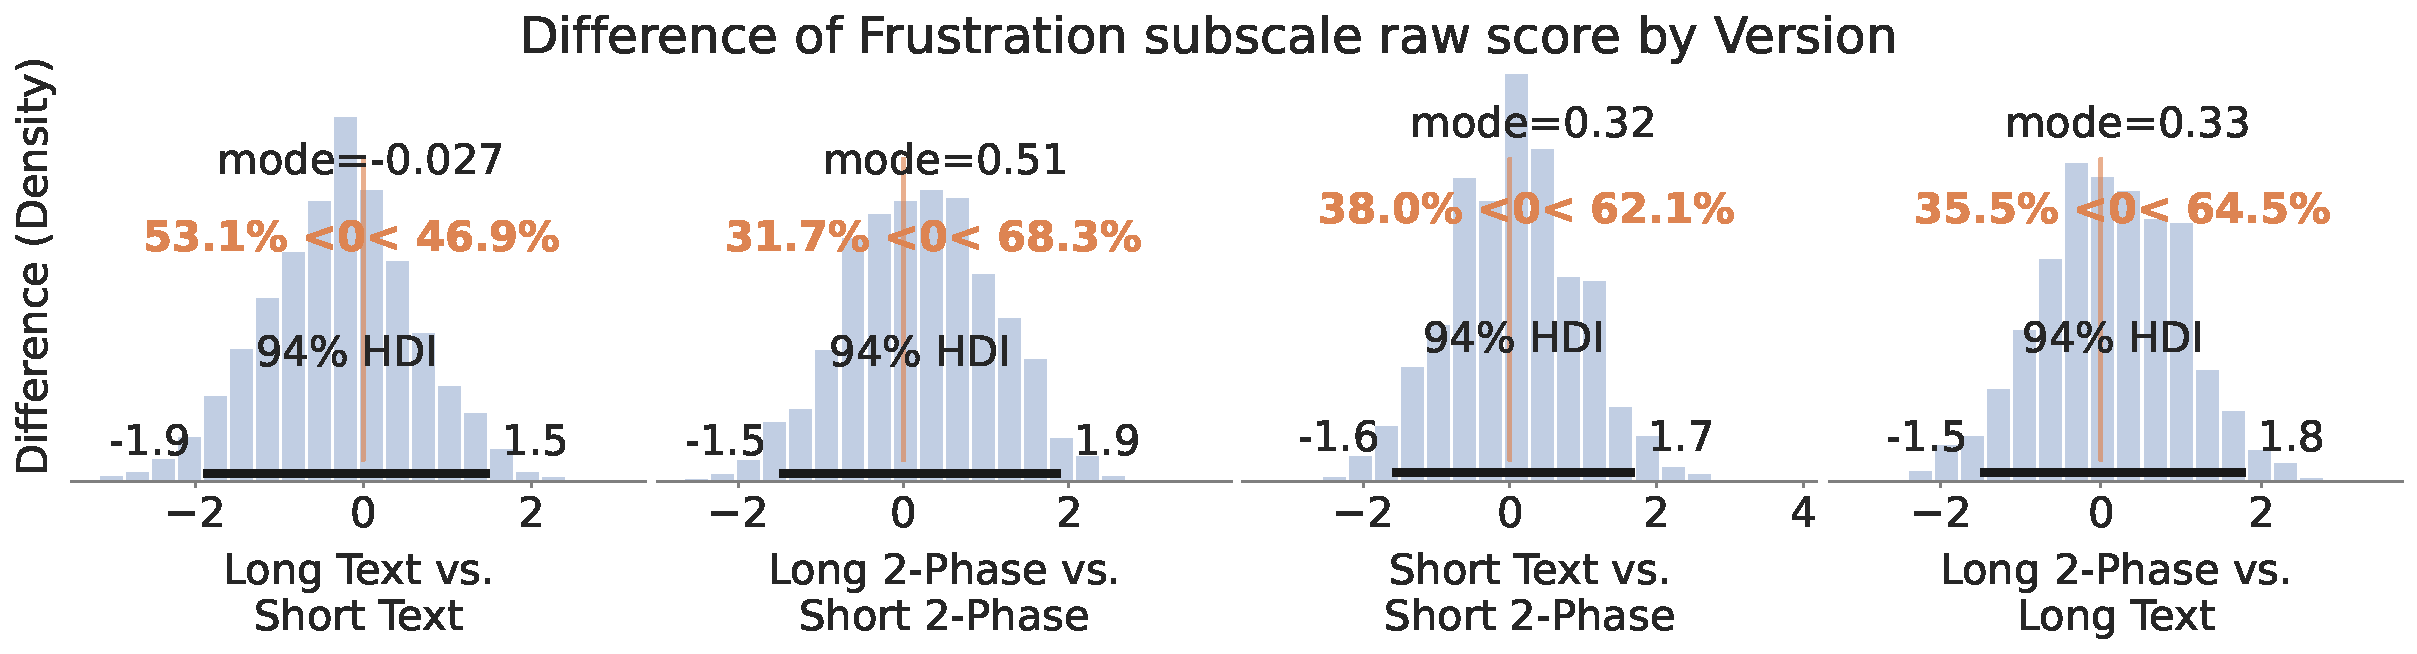
\includegraphics[width=\textwidth]{content/image/cog/Frustration_cog_diff_single_row.pdf}
    \caption{Differences in the frustration subscale scores by version.}
    \label{fig:bayesian_frustration_subscale}
\end{figure}
